\section{Feature Extraction Framework}\label{sec:features}

In this section, we present our framework to extract features designed to have two major characteristics: First, it effectively considers the heterogeneity of the network and regards its impact on the link formation time. Second, it takes the temporal dynamics of the network into account and leverages the network evolution history instead of simply aggregating it into a single snapshot. Here, we begin by formally defining the concepts of heterogeneous and dynamic information networks.

\begin{definition}[Heterogeneous Information Network]
An information network is \emph{heterogeneous} if it contains multiple kinds of nodes and links.
%Formally, it is defined as a directed graph $G=(V,E)$ where $V = \bigcup_i V_i$ is the set of nodes comprising the union of all the node sets $V_i$ of type $i$. Similarly, $E=\bigcup_j E_j$ is the set of links constituted by the union of all the link sets $E_j$ of type $j$.
A heterogeneous network is associated with a \emph{network schema} \cite{sun2011pathsim} which is used to describe it at a meta-level. It is a graph $\mc{S}_G=(\mc{V}, \mc{E})$ where $\mc{V}$ is the set of different node types and $\mc{E}$ is the set of different link types.
\end{definition}

\begin{definition}[Dynamic Information Network]
An information network is \emph{dynamic} when its nodes and linkage structure can change over time. That is, all nodes and links are associated with a birth and death time. More formally, a dynamic network at the timestamp $\tau$ is defined as $G^{\tau}=(V^{\tau}, E^{\tau})$ where $V^{\tau}$ and $E^{\tau}$ are respectively the set of nodes and the set of links existing in the network at the timestamp $\tau$.
\end{definition}

In this paper, we focus on two different heterogeneous and dynamic networks: (1) Delicious bookmarking network; and (2) MovieLens recommendation network. The schema of both these networks is depicted in Fig.~\ref{fig:schema}. %As an example, in Delicious network, $\mc{V}=\left\lbrace {User}, {Bookmark}, {Tag}\right\rbrace$ is the set of different node types, and $\mc{E}=\left\lbrace\text{contact}, \text{post}, \text{has-tag}\right\rbrace$ is the set of different link types. Whenever a user posts a new bookmark, a \emph{Bookmark} node will be added to the network, alongside with its corresponding new \emph{Tag} nodes (if they don't exist yet). New links will be formed among these newly added nodes to indicate \textit{post} and \textit{has-tag} relationships.


\begin{figure}
	\centering
	\scriptsize
	\tikzstyle{block} = [ellipse,draw=black]
	\tikzstyle{arrow} = [thick,->,>=stealth]
	\tikzstyle{label} = [fill=white,inner sep=0,xshift=0.1cm,yshift=.03cm]
	\tikzstyle{self} = [out=-110,in=-70,loop,shorten >=1pt]
	%	\subfloat[DBLP\label{fig:schema:dblp}]{
	%		\begin{tikzpicture}
	%		\node[block] (P) at (0,0) {$\underline{P}aper$};
	%		\node[block] (V) at (0,1) {$\underline{V}enue$};
	%		\node[block] (T) at (-2.4,0) {$\underline{T}erm$};
	%		\node[block] (A) at (2.4,0) {$\underline{A}uthor$};
	%		\node(hidden) [draw=none] at (0,-1){};
	%		
	%		\draw [arrow] (A) -- node[label] {write}   (P);
	%		\draw [arrow] (V) -- node[label] {publish} (P);           
	%		\draw [arrow] (P) -- node[label] {mention} (T);
	%		\draw [arrow] (P) to [self] node[label,yshift=-.2cm] {cite} (P);
	%		
	%		\end{tikzpicture}
	%	}
	%	\hfil
	\subfloat[MovieLens\label{fig:schema:movielens}]{
		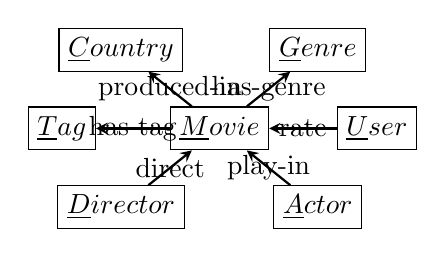
\begin{tikzpicture}
		
		\node[block] (M) at (0,0) {$\underline{M}ovie$};
		\node[block] (U) at (2.0,0) {$\underline{U}ser$};
		\node[block] (C) at (-1.25,1) {$\underline{C}ountry$};
		\node[block] (T) at (-2.0,0) {$\underline{T}ag$};
		\node[block] (G) at (1.25,1) {$\underline{G}enre$};
		\node[block] (A) at (1.25,-1) {$\underline{A}ctor$};
		\node[block] (D) at (-1.25,-1) {$\underline{D}irector$};
		\node(hidden) [draw=none] at (0,-1){};
		
		\draw [arrow] (U) -- node[label] {rate} (M);
		\draw [arrow] (M) -- node[label] {has-tag} (T);
		\draw [arrow] (M) -- node[label] {has-genre} (G);
		\draw [arrow] (A) -- node[label] {play-in} (M);
		\draw [arrow] (D) -- node[label] {direct} (M);
		\draw [arrow] (M) -- node[label] {produced-in} (C);
		
		\end{tikzpicture}
	}
	\hfil
	\subfloat[Delicious\label{fig:schema:delicious}]{
		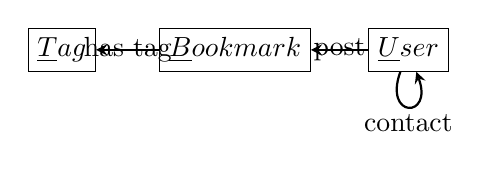
\begin{tikzpicture}
		
		\node(B) [block] at (0,0) {$\underline{B}ookmark$};
		\node(T) [block] at (-2.2,0) {$\underline{T}ag$};
		\node(U) [block] at (2.2,0) {$\underline{U}ser$};
%		\node(hidden) [draw=none] at (0,-1){};
		
		\draw [arrow] (U) -- node[label]{post} (B);
		\draw [arrow] (B) -- node[label]{has-tag} (T);
		\draw [arrow] (U) to [self] node[label,yshift=-.2cm]{contact} (U);
		
		\end{tikzpicture}
		%		\vspace{1cm}
	}
	
	\caption{Schema of three different heterogeneous networks. Underlined characters are used as abbreviations for corresponding node types. }
	\label{fig:schema}
\end{figure}



\begin{figure}
	\definecolor{blue}{HTML}{84CECC}
	\definecolor{darkblue}{HTML}{375D81}
	\definecolor{green}{HTML}{3F7F47}
	\begin{chronology}[align=left, startyear=0,stopyear=200, width=\columnwidth, height=1pt, startdate=false, stopdate=false, arrowwidth=4pt, arrowheight=3pt]
		\scriptsize
		\chronoevent[date=false]{10}{$t_0$}
		\chronoevent[date=false]{40}{$t_0+\Delta$}
		\chronoevent[date=false]{70}{$t_0+2\Delta$}
		\chronoevent[date=false,mark=false]{100}{$\dots$}
		\chronoevent[date=false]{130}{$t_0+k\Delta$}
		\chronoevent[date=false]{190}{$t_1$}
		\chronoperiode[color=darkblue, startdate=false, bottomdepth=2pt, topheight=5pt, textdepth=8pt, stopdate=false]{10}{40}{$\Delta$}
		\chronoperiode[color=blue, startdate=false, bottomdepth=10pt, topheight=15pt, textdepth=-15pt, stopdate=false]{10}{129}{Feature Extraction Window $(\Phi=k\Delta)$}
		\chronoperiode[color=green, startdate=false, bottomdepth=10pt, topheight=15pt, textdepth=-15pt, stopdate=false]{131}{190}{Observation Window $(\Omega)$}
	\end{chronology}
	\caption{The evolutionary timeline of the network data.}
	\label{fig:timeline}
\end{figure}

\subsection{Data Preparation For Feature Extraction}
To solve the problem of continuous-time link prediction in dynamic networks, we need to pay attention to the temporal history of the network data from two different points of view. First, we have to mind the evolution history of the network for feature extraction, so that the extracted features reflect the changes made in the network over time. Second, we have to specify the exact link formation time for each pair of nodes, because our goal is to propose a supervised method to predict a continuous variable, which in this case is the link formation time. Hence, for each sample pair of nodes, we need a feature vector $\mb{x}$, associated with a target variable $t$ indicating the formation time of the link between them.

Suppose that we have observed a dynamic network $G^{\tau}$ recorded in the interval $t_0 <\tau\le t_1$. According to Fig~\ref{fig:timeline}, we split this interval into two parts: the first part for extracting the feature $\mb{x}$, and the second for determining the target variable $t$. We refer to the first interval as \emph{Feature Extraction Window} whose length is denoted by $\Phi$, and the second as \emph{Observation Window}, whose length is denoted by $\Omega$. Now, based on the existence in the observation window, network links fall within one of the following three different groups:

\begin{enumerate}[label=(\roman*)]
	\item Links that have been formed in the feature extraction window (before the beginning of the observation window).
	\item Links that will be formed in the observation window for the first time (not existing before).
	\item Links that will not be formed at all (neither in the feature extraction window nor in the observation window).
\end{enumerate}

Links in the 2nd and 3rd categories constitute our data samples, and will be used in the learning procedure. For such links, we extract their feature vector $\mb{x}$ using the history available in the feature extraction window. For each link in the 2nd category, we see that it has been created at a time like $t_r\in(t_0+\Phi,t_1]$. So we set $t=t_r-(t_0+\Phi)$ as the time it takes for the link to form since the beginning of the observation window. For these samples, we also set an auxiliary variable $y=1$ which indicates that we have \emph{observed} their exact building time. On the other hand, we haven't seen the exact formation times of the links in the 3rd category, but we know that it should be definitely after $t_1$. For such \emph{censored} samples, we set $t=t_1-(t_0+\Phi)$ that is equal to the length of the observation window $\Omega$, and set $y=0$ to indicate that the recorded time is in fact a lower bound on the true link formation time. These type of samples are also of interest because their features will give us some information about their time falling after $t_1$. As a result, each sample is associated with a triple $(\mb{x},y,t)$ representing its feature vector, observation status, and the time it takes for the link to form, respectively.

%In Section \ref{sec:method}, we propose \npglm which is a supervised method to relate $x_l$ to $t_l$ by estimating $f_T(t_l\mid x_l)$ in a non-parametric fashion.

%Here is an toy example in a bibliographic network: Suppose that we have the data of the papers published between the years 1990 and 2010. For all papers, we have their authors, venue (where they are published), indexing terms, and their references. For each author pair, the goal is to predict by when one of them will cite another, if she has not done yet. To this end, we pick an intermediary year such as 2000 as pivot, and split the the data into two part. The paper that are published just before the year 2000 will belong to the feature extraction window, and the rest of the papers will fall within observation window. Now, for each pair of authors who did not cite each other in feature extraction window which 

\begin{table}[t]
	\centering
	\caption{Similarity Meta-Paths in Different Networks}
	\label{table:meta}
	\scriptsize
%	\setlength\tabcolsep{0pt}
	\begin{tabu} to \columnwidth {c c X[l]}
		\toprule
		Network & Meta-Path & Semantic Meaning \\
		\midrule
%		\multirow{6}{*}{\rotatebox{90}{DBLP}} 
%%		&&\\
%		& $A\rightarrow P\leftarrow A$ & Authors co-write a paper\\
%		& $A\rightarrow P\rightarrow A\leftarrow P\leftarrow A$ & Authors have common co-author\\
%		& $A\rightarrow P\rightarrow V\leftarrow P\leftarrow A$ & Authors publish in the same venue\\
%		& $A\rightarrow P\rightarrow T\leftarrow P\leftarrow A$ & Authors use the same term\\
%		& $A\rightarrow P\rightarrow P\leftarrow P\leftarrow A$ & Authors cite the same paper\\
%		& $A\rightarrow P\leftarrow P\rightarrow P\leftarrow A$ & Authors are cited by the same paper\\
%%		&&\\
%		\midrule
		\multirow{3}{*}{\rotatebox{90}{Delicious}} 
%		&&\\
		& $U\leftrightarrow U\leftrightarrow U$ & Users have common contact\\
		& $U\rightarrow B\leftarrow U$ & Users post the same bookmark\\
		& $U\rightarrow B\rightarrow T\leftarrow B\leftarrow U$ & Users post bookmarks with the same tag\\[0.05cm]
%		&&\\
		\midrule
		\multirow{11}{*}{\rotatebox{90}{MovieLens}} 
%		&&\\
		& $M\rightarrow A\leftarrow M$ & Movies share an actor\\
		& $M\rightarrow C\leftarrow M$ & Movies belong to the same country\\
		& $M\rightarrow D\leftarrow M$ & Movies have the same director\\
		& $M\rightarrow G\leftarrow M$ & Movies have the same genre\\
		& $M\rightarrow T\leftarrow M$ & Movies have the same tag\\
%		\cmidrule{2-3}
		& $U\rightarrow M\leftarrow U$ & Users rate common movie\\
		& $U\rightarrow M\rightarrow A\leftarrow M\leftarrow U$ & Users rate movies sharing an actor\\
		& $U\rightarrow M\rightarrow C\leftarrow M\leftarrow U$ & Users rate movies from the same country\\
		& $U\rightarrow M\rightarrow D\leftarrow M\leftarrow U$ & Users rate movies of the same director\\
		& $U\rightarrow M\rightarrow G\leftarrow M\leftarrow U$ & Users rate movies with the same genre\\
		& $U\rightarrow M\rightarrow T\leftarrow M\leftarrow U$ & Users rate movies with the same tag\\
%		&&\\
		\bottomrule
	\end{tabu}
\end{table}

\subsection{Dynamic Feature Extraction}
In this part, we describe how to utilize the temporal history of the network in the feature extraction window in order to extract features for continuous-time link prediction problem. We first begin with the meta-path-based feature set for heterogeneous information networks, and then incorporate these features into a \emph{recurrent neural network based autoencoder} to exploit the temporal dynamics of the network as well. Hereby, we begin by defining the concept of meta-path \cite{sun2011pathsim}:

\begin{definition}[Meta-Path]
	In a heterogeneous information network, a meta-path is a directed path following the graph of the network schema to describe the general relations that can be derived from the network. Formally, given a network schema $\mc{S}_G=(\mc{V}, \mc{E})$, the sequence $\nu_1\xrightarrow{\varepsilon_1}\nu_2\xrightarrow{\varepsilon_2}\dots\nu_{k-1}\xrightarrow{\varepsilon_{k-1}}\nu_k$ is a meta-path defined on $S_G$ where $\nu_i\in \mc{V}$ and $\varepsilon_i\in \mc{E}$.
\end{definition} 

Meta-paths are commonly used in heterogeneous information networks to describe multi-typed relations that have concrete semantic meanings. For example, in the MovieLens network, whose schema is show in Fig~\ref{fig:schema:movielens}, we model the relationship between different movies sharing the same director as the following meta-path:
\[Movie\xleftarrow{direct}Director\xrightarrow{direct}Movie\]
or simply as $M\leftarrow D\rightarrow M$.
%Another example is the author citation relation, which in this paper is used as the target relation for DBLP network. It can be specified as:
%\[Author\xrightarrow{write}Paper\xrightarrow{cite}Paper\xleftarrow{write}Author\]
%abbreviated as $A\rightarrow P\rightarrow P\leftarrow A$.
Among the possible meta-paths that can be defined on a network schema, there are some that capture the similarity between two nodes. For example, the aforementioned meta-path $M\leftarrow D\rightarrow M$ in MovieLens network creates a sense of similarity between two \emph{Movie} nodes. These type of meta-paths, called \emph{similarity meta-paths}, are widely used to define topological features for link prediction problem in heterogeneous networks \cite{sun2011co, 7752228}. Table~\ref{table:meta} presents a number of similarity meta-paths that can be defined on Delicious and MovieLens networks to capture the heterogeneous similarity between different node types.

The concept of similarity meta-paths can be extended to define heterogeneous features suitable for link prediction problem. Here we follow the same approach as in \cite{sun2012will} which suggests triple building blocks to describe features for link prediction problem, given a certain link type $\varepsilon$ as the target link type to be predicted between two nodes of type $A$ and $B$: 
\begin{enumerate}
	\small
	\item $A\rightsquigarrow A\rightarrow B$, where $\rightsquigarrow$ and $\rightarrow$ denote similarity meta-path and the target link, respectively. This block tells that a node of type $A$ is similar to another node of the same type, which itself forms a link of type $\varepsilon$ with a node of type $B$. Thus, those similar nodes may also link to the type $B$ node.
	\item $A\rightarrow B \rightsquigarrow A$, which has a similar intuition as the first block.
	\item $A\rightsquigarrow C \rightsquigarrow B$, saying that some nodes of type $A$ are in relation with some type $C$ nodes, which are themselves in relation with some nodes of type $B$. Hence, it is likely that type $A$ nodes form some links, such as the target link, with type $B$ nodes.
\end{enumerate}
%where $\rightsquigarrow$ denotes a similarity meta-path, and $A\rightarrow B$ is a link of type $\varepsilon$. The first block tells that a node of type $A$ is similar to another node of the same type, which itself has a relationship of type $\varepsilon$ with a node of type $B$. Therefore, those similar nodes may also form the target relation with the type $B$ node. An analogous intuition is behind the second block. For the third, it says that some nodes of type $A$ are in relation with some type $C$ nodes, which are themselves in relation with some nodes of type $B$. Hence, it is likely that type $A$ nodes form some links, such as the target link, with type $B$ nodes.

%As an example in DBLP bibliographic network, for the target relation we use $A\rightarrow P\rightarrow P\leftarrow A$ as the meta-path denoting the author citation relation. In Addition, Paper-cite-Author ($P\rightarrow P\rightarrow A$) and Author-cite-Paper ($A\rightarrow P\rightarrow P$) are also used as the arbitrary relations, and the similarity meta-paths for DBLP network from Table~\ref{table:meta} are used to define the features for author citation link prediction.

After specifying the suitable meta-paths, we need a method to quantify them as features, considering the dynamicity of the network. Here, we formally define \emph{time-aware meta-path-based features}:

\begin{definition}[Time-Aware Meta-Path-based Feature]
	Suppose that we are given a dynamic heterogeneous network $G^{\tau}$ along with its network schema $\mc{S}_G=(\mc{V}, \mc{E})$, and a target link type $A\rightarrow B$. For a given pair of nodes $a\in A$ and $b\in B$, and a meta-path $\Psi=\nu_1\xrightarrow{\varepsilon_1}\nu_2\xrightarrow{\varepsilon_2}\dots\nu_{k-1}\xrightarrow{\varepsilon_{k-1}}\nu_k$ defined on $\mc{S}_G$, the time-aware meta-path-based feature at the timestamp $\tau$ is:
	\begin{equation*}
		\begin{split}
			&f_{\Psi}^\tau(a,b)=I(a,A)I(b,B)\\
			&\sum_{n_1\in\nu_1,\dots,n_k\in\nu_k}\prod_{i=1}^{k-1}\mb{1}\Big((n_i,n_{i+1})\in\varepsilon_i\Big)\mb{1}\Big(bt(n_i,n_{i+1}) < \tau \le dt(n_i,n_{i+1})\Big)
		\end{split}
	\end{equation*}
	where $\mb{1}(.)$ is the binary predicate function, and $bt(n_i,n_{i+1})$ and $dt(n_i,n_{i+1})$ denote the birth and the death time of the link $(n_i,n_{i+1})$, respectively.
\end{definition}

By using the above definition, we will be able to quantify the number of instances of any particular meta-path at any specific timestamp. If we set this timestamp to the end of the feature extraction window, it is as though we are aggregating the whole network into a single snapshot observed at time $t_0+\Phi$. In order to avoid such an aggregation, we divide the feature extraction window into a sequence of $k$ contiguous intervals of a constant size $\Delta$, as shown in Fig.~\ref{fig:timeline}. By doing so, we intend to extract time-aware features in each sub-window that results in a multivariate time series containing the information about the temporal evolution of the topological features between any pair of nodes. With this in mind, we define \emph{dynamic meta-path-based time series}:

\begin{definition}[Dynamic Meta-Path-based Time Series]
	Suppose that we are given a dynamic heterogeneous network $G^{\tau}$ observed in a feature extraction window of size $\Phi$ ($t_0<\tau \le t_0+\Phi$), along with its network schema $\mc{S}_G=(\mc{V}, \mc{E})$ and a target relation $A\rightarrow B$. Also suppose that the feature extraction window is divided into $k$ fragments of size $\Delta$. For a given pair of nodes $a\in A$ and $b\in B$ in $G^{t_0+\Phi}$, and a meta-path $\Psi$ defined on $\mc{S}_G$, the dynamic meta-path-based time series of $(a,b)$ is:
	\begin{equation*}
		x_{\Psi}^i(a,b)=f_{\Psi}^{t_0+i\Delta}(a,b) - f_{\Psi}^{t_0+(i-1)\Delta}(a,b)\quad\quad i=1\dots k
	\end{equation*}
\end{definition}

For each unique meta-path, we get a unique time series. For each time step, we put the corresponding values from all time series into a vector. Consequently, we get a multivariate time series where each time step is vector-valued. For example, if we have $d$ meta-paths $\Psi_1$ to $\Psi_d$, then each time step of the resulting time series will be of the form $\mb{x}^i=[x_{\Psi_1}^i,\dots,x_{\Psi_d}^i]^T$. Such multivariate time series reflect how topological features between two nodes change across different snapshots of the network, and can capture increasing/decreasing trends or even periodic/re-occurring patterns.

Now it's the time to convert this multivariate time series into a single feature vector so that we can use it as the input of our non-parametric model that is discussed in the next section. A trivial solution would be to stack all vectors of the multivariate time series into a single one, and feed our model with this single vector. However, this approach will result in a very high dimensional vector as the number of time steps increases, and can lead to difficulties in the learning procedure due to the curse of dimensionality. This is in contrast with our expectation that more time steps means more information about the history of the network and should result in a better prediction model. To overcome this problem, we combine the power of recurrent neural networks, especially Long Short Term Memory (LSTM) units \cite{hochreiter1997long}, which have proven to be very successful in handling time series and sequential data, with autoencoders \cite{bengio2009learning}, which are widely used to learn alternative representations of the data such that the learned representation can reconstruct the original input.

\begin{figure}
	\centering
	\footnotesize
	\tikzstyle{block} = [rectangle,draw=black,minimum width=0.5cm, minimum height=0.25cm]
	\tikzstyle{arrow} = [thick,->,>=stealth]
	\tikzstyle{label} = [rectangle]
	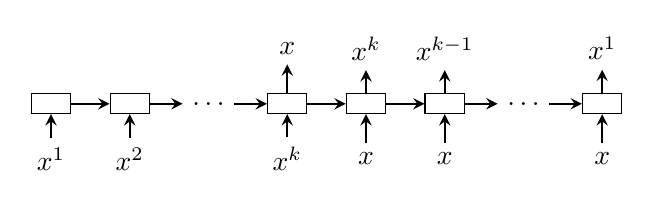
\begin{tikzpicture}
	\node[block] (e1) at (0,0) {};
	\node[block] (e2) at (1,0) {};
	\node[block,draw=none] (ed) at (2,0) {$\dots$};
	\node[block] (ek) at (3,0) {};
	
	\node[block] (dk) at (4,0) {};
	\node[block] (dk1) at (5,0) {};
	\node[block,draw=none] (dd) at (6,0) {$\dots$};
	\node[block] (d1) at (7,0) {};
	
	\node[label] (ie1) at (0,-0.7) {${x}^1$};
	\node[label] (ie2) at (1,-0.7) {${x}^2$};
	\node[label] (iek) at (3,-0.7) {${x}^k$};
	
	\node[label] (idk) at (4,-0.7) {$\mb{x}$};
	\node[label] (idk1) at (5,-0.7) {$\mb{x}$};
	\node[label] (id1) at (7,-0.7) {$\mb{x}$};
	
	\node[label] (oek) at (3,0.7) {$\mb{x}$};
	\node[label] (odk) at (4,0.7) {${x}^k$};
	\node[label] (odk1) at (5,0.7) {${x}^{k-1}$};
	\node[label] (od1) at (7,0.7) {${x}^1$};
	
	\draw [arrow] (ie1) -- (e1);
	\draw [arrow] (ie2) -- (e2);
	\draw [arrow] (iek) -- (ek);
	
	\draw [arrow] (idk) -- (dk);
	\draw [arrow] (idk1) -- (dk1);
	\draw [arrow] (id1) -- (d1);
	
	\draw [arrow] (ek) -- (oek);
	\draw [arrow] (dk) -- (odk);
	\draw [arrow] (dk1) -- (odk1);
	\draw [arrow] (d1) -- (od1);
	
	\draw [arrow] (e1) -- (e2);
	\draw [arrow] (e2) -- (ed);
	\draw [arrow] (ed) -- (ek);
	\draw [arrow] (ek) -- (dk);
	\draw [arrow] (dk) -- (dk1);
	\draw [arrow] (dk1) -- (dd);
	\draw [arrow] (dd) -- (d1);
	
	\end{tikzpicture}
	\caption{The architecture of LSTM autoencoder for dynamic feature extraction. The learned representation of the $k^{\text{th}}$ stage is used as the feature $\mb{x}$.}
	\label{fig:autoencoder}
\end{figure}

Inspired by the work of Dai and Le on semi-supervised sequence learning \cite{dai2015semi}, we design an LSTM autoencoder which takes a multivariate time series as input, and tries to encode it to a latent representation, so that it can then predict the input time series from the learned vector. The architecture of such autoencoder is illustrated in Fig~\ref{fig:autoencoder}. The benefits of using this autoencoder is two-fold: (1) since the autoencoder can reconstruct the original time series, which reflects the temporal dynamics of the network, we get minimum information loss in the learned vector; and (2) as we can set the dimensionality of the encoded vector to any desired value, we can evade the curse of dimensionality. We explain our proposed non-parametric model in the next section that takes the learned representation as the feature vector $\mb{x}$ and attempts to predict the corresponding time $t$. 


